\chapter{The cohomology of decomposition spaces}\label{chapter:decomposition_spaces}

Epstein asked whether there is an algorithm that, when given a presentation for a hyperbolic group $G$, computes the \vCech{} cohomology $\cH{}^k(\boundary G)$ as a $G$-module.
This problem appears as Question 1.18{} in Bestvina's problem list~\cite{bestvina}.
Throughout this chapter all \vCech{} cohomology groups will have coefficients in $\integers$, although most of the results given apply to other rings.
Our purpose in this chapter is to answer a relative version of this question in the case of Otal's decomposition space, a special case of the Bowditch boundary of a relatively hyperbolic group.
We then apply this result to answer Epstein's question for a restricted class of hyperbolic groups: those arising as fundamental groups of graphs of free groups with cyclic edge groups.

Fix a free group $F$ of rank $n$ with free generating set $S$.
Let $T$ be the corresponding Cayley graph containing a vertex $1$ corresponding to the identity in $F$.
Fix a finite set $\{w_i\}$ of cyclically reduced words in $F$.
Then, following Otal~\cite{otal92}, we make the following definitions.

\begin{definition}
  The \emph{line pattern $\calL$} associated to the set $\{w_i\}$ is defined to be the set of lines spanned by the points\/ $\{gw_i^k\}_k$ for\/ $g \in F$.
  Let\/ $\calD$ be the associated \emph{decomposition space}: this is the quotient of\/ $\boundary F$ by the equivalence relation that identifies the two end points of each line in\/ $\calL$.
  Let\/ $q \colon \boundary F \to \calD$ be the quotient projection.
\end{definition}

If we assume that each of the elements of $\{w_i\}$ is not a proper power and that for distinct $i$ and $j$ the element $w_i$ is not conjugate in $F$ to $w_j^{\pm}$ then $\calD$ is the Bowditch boundary of group $F$ relative to $\{\langle w_i\rangle\}$ by a result of Tran~\cite{tran13}: see Theorem~\ref{theorem:bowditch_from_gromov}.

We present an algorithm that computes the \vCech{} cohomology of $\calD$ as an $F$-module.
The $F$-module structure is induced by the action of $F$ on $\boundary F$, which descends to an action of $F$ on $\calD$.
The cohomology functor is contravariant, so we use the action of $g^{-1}$ on $\calD$ to define the action of $g$ on $\cH{}^k(\calD)$.
Given $g \in F$ let $\phi_g$ be the corresponding homeomorphism of $\calD$.
Then we define the action of $g$ on $\cH{}^k(\calD)$ by setting $g \cdot x = (\phi_{g^{-1}})^\star x$.

The \vCech{} cohomology of $\calD$ is defined to be the direct limit over open covers $\calU$ of $\calD$ that provide successively better combinatorial approximations to $\calD$ of the singular cohomology of the nerve of $\calU$.
In Section~\ref{section:whitehead_diagrams} we shall see how to associate an open cover of $\calD$ to a finite subtree of $T$.
The combinatorics of such a cover will then be recorded in the Whitehead graph associated to that subtree.
Therefore Whitehead graphs provide approximations to $\calD$, with larger Whitehead graphs providing better approximations.

These open covers have no triple intersections, so we immediately see that the \vCech{} cohomology is concentrated in dimensions zero and one.
This could also be seen as a consequence of the Urysohn--Menger addition theorem~\cite[3.1.17]{engelking78}: if $X$ is a compact metric space and $A$ and $B$ are subsets of $X$ with $X = A \union B$ then $\dim X \leq \dim A + \dim B + 1$ where $\dim$ is the Lebesgue covering dimension.
The decomposition space $\calD$ can be written as a union of the set of points in $\boundary F$ that are not end points of lines in $\calL$ with the set of images in $\calD$ of end points of lines in $\calL$.
The first of these sets is a subset of a Cantor set, so has dimension zero, while the second is countable, so also has dimension zero, thus proving that $\calD$ has dimension at most one.

In Sections~\ref{section:dimension_0_cohomology} and~\ref{section:dimension_1_cohomology} we show how to compute the \vCech{} cohomology in dimensions zero and one respectively.
In dimension zero this could be accomplished by computing a maximal free splitting of the group relative to the set $\{\langle w_i\rangle\}$ of subgroups of $F$ and then relating the decomposition space to the tree associated to the splitting; in Section~\ref{section:graphs_of_free_groups} we apply an argument along these lines.
In Section~\ref{section:dimension_0_cohomology} we take an alternative approach: our methods rely on showing that some (large) finite subtree of $T$ contains sufficient information to compute the \vCech{} cohomology.
This approach is based on the proof of \cite[Lemma 4.12]{cashenmacura11}.

In Section~\ref{section:graphs_of_free_groups} we apply these results to prove the computability of the \vCech{} cohomology of the boundary of a hyperbolic fundamental group of a graph of free groups with virtually cyclic edge groups.
This result answers Epstein's question for this restricted class of hyperbolic groups.

\section{Whitehead graphs and open covers}\label{section:whitehead_diagrams}

Recall the following definition from~\cite{cashenmacura11}.

\begin{definition}
  Let $X$ be a subtree of $T$.
  Then we define the \emph{Whitehead graph $\Wh{X}$ of $\calL$ at $X$} to be the graph with a vertex corresponding to each vertex of $T$ adjacent to (but not contained in) $X$ and an edge connecting a pair of vertices in $\Wh{X}$ for each line in $\calL$ connecting the corresponding vertices in $T$.
  The edges of $\Wh{X}$ are labelled by the corresponding lines.
\end{definition}

For more information about Whitehead graphs and their applications, see~\cite{manning10}.

\begin{definition}
  For $v \in T$ let $\shadow_1(v) \subset \boundary T$ be the \emph{shadow} of $v$ from $1$ as defined in~\cite{cashenmacura11}: the set of boundary points $p \in \boundary T$ such that the geodesic $[1, p]$ contains $v$.
  These sets are open and closed and the collection of such sets as $v$ varies in $T$ is a basis for the topology on $\boundary T$.
\end{definition}

\begin{lemma}\label{lemma:constructing_a_cover}
  Let $X$ be a finite subtree of\/ $T$ containing $1$.
  Then there is a covering of\/ $\calD$ by a collection of open sets $U_i$ in bijection with the vertices $a_i$ of\/ $\Wh{X}$ satisfying the following conditions.
\begin{itemize}
  \item The projection of\/ $\shadow_1(a_i)$ to\/ $\calD$ is a subset of\/ $U_i$.
  \item The pairwise intersections of sets in the cover can be read from the Whitehead diagram: $U_i \intersection U_j \neq \emptyset$ if and only if there is an edge connecting $a_i$ and $a_j$ in $\Wh{X}$.
  \item There are no triple intersections.
  \end{itemize}
\end{lemma}

\begin{proof}
We aim to construct open sets $V_i$ covering $\boundary T$ satisfying the following conditions.
\begin{itemize}
  \item The shadow $\shadow_1(a_i)$ is contained in $V_i$.
  \item Intersections are determined by the Whitehead graph: $V_i \intersection V_j \neq \emptyset$ if and only if there is an edge connecting $a_i$ and $a_j$ in $\Wh{X}$.
  \item There are no triple intersections.
  \item For each line $l$ in the line pattern $\calL$, each set $V_i$ contains either both of the end points of $l$ or neither.
\end{itemize}
Then the projection of these sets in $\calD$ satisfies the requirements of the lemma.

We build these inductively.
For the first step, take $V_i^0 = \shadow_1(a_i)$.
Then, for each $i$, there are finitely many lines in the line pattern passing through $a_i$.
Add to $V_i^0$ an open neighbourhood of the end point not in $V_i^0$ of each such line to obtain $V_i^1$.
This can be done in a way that ensures that $V_i^1$ is the union of $V_i^0$ and finitely many other shadows, that the open sets added are all disjoint, and that no line in the line pattern has an end in two different added sets.
This is possible since if a subset of $\boundary T$ is a union of finitely many shadows then only finitely many lines in the line pattern have exactly one end in that subset.

After each $V_i^1$ is defined, continue inductively, ensuring that each $V_i^k$ is the union of finitely many shadows, so that if a line in the line pattern has one end in $V_i^k$ then its other end is in $V_i^{k+1}$.
We can do this without introducing any new intersections, so all intersections correspond to lines from $\shadow_1(a_i)$ to $\shadow_1(a_j)$ for some $i$ and $j$, so all intersections correspond to edges in the Whitehead graph and there are no triple intersections.

Then let $U_i = q(\union_k V_i^k)$; these sets cover $\calD$ and have the required properties.
\end{proof}

For $X$ a finite subtree of $T$, we shall denote by $\calU_X$ a cover of $\calD$ associated to $X$ as constructed in Lemma~\ref{lemma:constructing_a_cover}.
This cover is not unique, but this non-uniqueness will not cause us a problem, since any two such covers are very similar.
In particular, they admit a common refinement, and refinement between different open covers associated to $X$ as in Lemma~\ref{lemma:constructing_a_cover} induces a natural isomorphism between the singular cochain complexes of the nerves of those covers.
If $X \subset X'$ then $\calU_{X'}$ can be chosen to be a refinement of $\calU_X$ and the refinement map $\calU_{X'} \to \calU_X$ is canonical.

It will be convenient to define an open cover associated to the empty subtree of $X$: this is the trivial covering $\calU_\emptyset = \{\calD\}$.

\begin{lemma}\label{lemma:refining}
  Let $\calW$ be a finite open cover of\/ $\calD$.
  Then some refinement of\/ $\calW$ is of the form given in Lemma~\ref{lemma:constructing_a_cover}.
\end{lemma}

\begin{proof}
Let $\calV$ be the pullback of $\calW$ to $\boundary T$. Consider the set
\begin{align}
  C = \{a \in T \vert \shadow_1(a) \subset V \text{ for some } V \in \calV\}.
\end{align}

The collection $\{\shadow_1(x) \vert x \in T\}$ is a basis for the topology on $\boundary T$ so sets of the form $\shadow_1(a)$ for $a\in C$ cover each $V \in \calV$.
Hence such sets cover $\boundary T$.

The boundary $\boundary T$ is compact, so there is a finite set of points $a_1, \dots , a_n$ such that $\{\shadow_1(a_i) \}$ covers $\boundary T$ and each $\shadow_1 (a_i)$ is contained in some $V_{\sigma(i)} \in \calV$.
Let $H$ be the convex hull of $\{a_i\} \union \{1\}$.
Call vertices of $H$ adjacent to vertices in $T - H$ boundary vertices.
If we take $\{a_i\}$ to be minimal with its covering property then the set of boundary points of $H$ is precisely $\{a_i\}$.
Let $X$ be the subtree of $H$ obtained by pruning off its boundary vertices.

Let $\calU_X = \{U_i\}$ be the finite cover of $\calD$ corresponding to $X$ as in Lemma~\ref{lemma:constructing_a_cover}.
Define a new set $\calU'$ of open subsets of $\calD$ by
\begin{align}
  \calU' = \{U_i \intersection q(V_{\sigma(i)})\}.
\end{align}

The set $\calU'$ is a cover of $\calD$ since it covers $q(\shadow_1(a_i))$ for each $i$.
It is certainly a refinement of $\calW$ and it is easy to check that it corresponds to $X$ in the sense of the statement of Lemma~\ref{lemma:constructing_a_cover}.
\end{proof}

The results of this section together imply the following corollary:

\begin{corollary}
  The finite Whitehead diagrams determine the cohomology of $\calD$:
  \begin{align}
  \cH{}^n(\calD)= \directlimit_X\cH{}^n (\calU_X)
  \end{align}
  where the direct limit is taken over finite subtrees $X$ of $T$, partially ordered by inclusion.
\qed
\end{corollary}


\section{Computing \texorpdfstring{$\cH{}^0(\calD)$}{H0(D,Z)}}\label{section:dimension_0_cohomology}

For each element $[\sigma] \in \cH{}^0(\calD)$ there exists a subtree $X \subset T$ such that $[\sigma]$ is represented by some $\sigma \in \cH{}^0(\calU_X)= \ker\left( d^0 \colon \cC{}^0(\calU_X)\to \cC{}^1(\calU_X)\right)$.
Such an element is an assignment of an integer to each connected component of \Wh{X}.
In this situation we shall say that $[\sigma]$ is \emph{supported on $X$} and we shall refer to the minimal such subtree as the \emph{support of $[\sigma]$}.
A unique minimal such subtree exists: it is clear that if $[\sigma]$ is supported on $X_1$ and on $X_2$ then it is supported on $X_1 \intersection X_2$.

As discussed at the beginning of the chapter, $F$ acts on $\calD$ by homeomorphisms, giving the \vCech{} cohomology the structure of an $F$-module with $g$ acting as $\phi_{g^{-1}}^\star$ on $\cH{}^0(\calD)$.
In terms of Whitehead graphs, any $g\in F$ induces a map
\begin{align}
  g \colon \cH{}^0(\calU_X) \to \cH{}^0(g\cdot\calU_X)= \cH{}^0(\calU_{g(X)}).
\end{align}
This map takes an element represented by a $\integers$-labelling of the connected components of \Wh{X} to the element represented by the translate by $g$ of this labelled diagram.

We now aim to find an algorithm that computes a presentation for this $F$-module. First we describe an algorithm that computes a generating set.
The argument is loosely based on the proof of~\cite[Lemma 4.12]{cashenmacura11}.

\begin{proposition}\label{proposition:generators_0}
There exists a finite number $N$, computable from $n$ and $\calL$, such that $\cH{}^0(\calD)$ is generated as an abelian group by 0-cycles supported on subtrees of $T$ with at most $N$ vertices.
\end{proposition}

\begin{proof}
  Let $[\sigma]$ be a 0-cycle supported on a subtree $X$ of $T$ with more than $N$ vertices, where $N$ is to be chosen later.
  Then by induction it is sufficient to show that $[\sigma]$ can be written as the sum of 0-cycles supported on strictly smaller subtrees.
  The idea is that if $N$ is large enough then there will be two vertices in $X$ at which $[\sigma]$ looks similar and cutting out everything between these vertices allows us to split $[\sigma]$ into strictly smaller summands.

  $\cH{}^0(\calU_X)$ is generated by 0-cycles represented by Whitehead diagrams at $X$ with one connected component labelled 1 and the others labelled 0.
  We can assume without loss of generality that $[\sigma]$ is such a 0-cycle.
  Then $[\sigma]$ can be thought of as a partition of $\Wh{X}$ into a connected component and its complement.
  An example of such a partition is shown pictorially in Figure~\ref{fig:partition}.

\begin{figure}
\centering

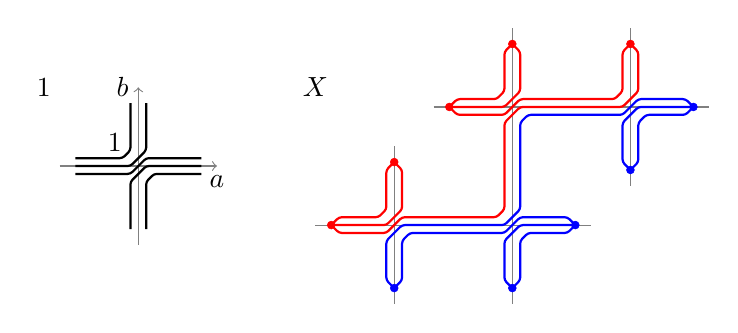
\begin{tikzpicture}[scale=1]

\begin{scope}[shift={(-2.75,0)}] % Frame for Wh(1)
  \begin{scope}[gray]
    \draw[->] (-1,0) -- (1,0) node[black,anchor=north] {\(a\)};
    \draw[->] (0,-1) -- (0,1) node[black,anchor=east] {\(b\)};
  \end{scope}

  \draw (-1.2,1) node {\(\Wh{1}\)}; %Label for left diagram
  \draw (-0.30,0.30) node {\(1\)}; %Label origin in Wh(1)

  \begin{scope}[thick,rounded corners=1pt] % Edges in Wh(1)
    \draw (-0.8,0.1) -- (-0.2,0.1) -- (-0.1,0.2) -- (-0.1,0.8);
    \draw (-0.8,0) -- (-0.1,0) -- (0.1,0.2) -- (0.1,0.8);
    \draw (-0.8,-0.1) -- (-0.1,-0.1) -- (0.1,0.1) -- (0.8,0.1);
    \draw (-0.1,-0.8) -- (-0.1,-0.2) -- (0.1,0) -- (0.8,0);
    \draw (0.1,-0.8) -- (0.1,-0.2) -- (0.2,-0.1) -- (0.8,-0.1);
  \end{scope}
\end{scope}

\begin{scope}[shift={(2,-0.75)}]

  \draw (-2.5,1.75) node {\(\Wh{X}\)}; % Label for right diagram

  \begin{scope}[gray] % Frame for Wh(X)
    \draw (-2.5,0) -- (1,0);
    \draw (-1,1.5) -- (2.5,1.5);
    \draw (-1.5,1) -- (-1.5,-1);
    \draw (0,2.5) -- (0,-1);
    \draw (1.5,2.5) -- (1.5,0.5);;
  \end{scope}

  \begin{scope} % Red vertices in Wh(X)
    [disc/.style={circle,draw=red,fill=red,very thin,inner sep=0pt,minimum
      size=1mm}]
    \node at (-0.8,1.5) [disc] {};
    \node at (0,2.3) [disc] {};
    \node at (1.5,2.3) [disc] {};
    \node at (-2.3,0) [disc] {};
    \node at (-1.5,0.8) [disc] {};
  \end{scope}

  \begin{scope} %Blue vertices in Wh(X)
    [disc/.style={circle,draw=blue,fill=blue,very thin,inner sep=0pt,minimum
      size=1mm}]
    \node at (-1.5,-0.8) [disc] {};
    \node at (0,-0.8) [disc] {};
    \node at (0.8,0) [disc] {};
    \node at (2.3,1.5) [disc] {};
    \node at (1.5,0.7) [disc] {};
  \end{scope}

  \begin{scope}[thick,red,rounded corners=1pt] % Red edges in Wh(X)
    \draw (-2.3,0) -- (-2.2,0.1) -- (-1.7,0.1) -- (-1.6,0.2) -- (-1.6,0.7)
      -- (-1.5,0.8);
    \draw (-2.3,0) -- (-1.6,0) -- (-1.4,0.2) -- (-1.4,0.7) -- (-1.5,0.8);
    \draw (-0.8,1.5) -- (-0.7,1.6) -- (-0.2,1.6) -- (-0.1,1.7) -- (-0.1,2.2)
      -- (0,2.3);
    \draw (-0.8,1.5) -- (-0.1,1.5) -- (0.1,1.7) -- (0.1,2.2) -- (0,2.3);
    \draw (-2.3,0) -- (-2.2,-0.1) -- (-1.6,-0.1) -- (-1.4,0.1) -- (-0.2,0.1)
      -- (-0.1,0.2) -- (-0.1,1.3) -- (0.1,1.5) -- (1.4,1.5) -- (1.6,1.7)
      -- (1.6,2.2) -- (1.5,2.3);
    \draw (-0.8,1.5) -- (-0.7,1.4) -- (-0.1,1.4) -- (0.1,1.6) -- (1.3,1.6)
      -- (1.4,1.7) -- (1.4,2.2) -- (1.5,2.3);
  \end{scope}

  \begin{scope}[thick,blue,rounded corners=1pt] % Blue edges in Wh(X)
    \draw (0,-0.8) -- (-0.1,-0.7) -- (-0.1,-0.2) -- (0.1,0) -- (0.8,0);
    \draw (0,-0.8) -- (0.1,-0.7) -- (0.1,-0.2) -- (0.2,-0.1) -- (0.7,-0.1)
      -- (0.8,0);
    \draw (1.5,0.7) -- (1.4,0.8) -- (1.4,1.3) -- (1.6,1.5) -- (2.3,1.5);
    \draw (1.5,0.7) -- (1.6,0.8) -- (1.6,1.3) -- (1.7,1.4) -- (2.2,1.4)
      -- (2.3,1.5);
    \draw (-1.5,-0.8) -- (-1.4,-0.7) -- (-1.4,-0.2) -- (-1.3,-0.1) -- (-0.1,-0.1)
      -- (0.1,0.1) -- (0.7,0.1) -- (0.8,0);
    \draw (-1.5,-0.8) -- (-1.6,-0.7) -- (-1.6,-0.2) -- (-1.4,0) -- (-0.1,0)
      -- (0.1,0.2) -- (0.1,1.3) -- (0.2,1.4) -- (1.4,1.4) -- (1.6,1.6)
      -- (2.2,1.6) -- (2.3,1.5);
  \end{scope}
\end{scope}

\end{tikzpicture}
\caption{\label{fig:partition}
  A partition of a disconnected Whitehead graph into two connected components.
  An assignment of the integer 1 to the red part and 0 to the blue part represents an element of $\cH{}^0(\calD)$.
  In this example $F$ is free on two generators and the line pattern is generated by the word $a^2bab$.
}
\end{figure}

Suppose that $N$ is large enough that any subtree of $T$ with more than $N$ vertices is guaranteed to contain an embedded arc of length at least $M+2$, where $M$ is a computable function of $n$ and $\calL$ to be chosen later.
Then let $v_1, \ldots, v_M$ be the interior vertices of such an embedded arc in $X$.
Traversing this arc in the direction from $v_1$ to $v_M$, record for each vertex $v_i$ an ordered pair $(s_i, t_i)$ of elements of $S^\pm$, where $s_i$ labels the incoming edge at $v_i$ of the embedded arc at and $t_i$ labels the outgoing edge.

Suppose that $M$ is large enough that at least $K$ of these pairs are equal.
Here $K$ is a computable function of $\calL$ to be chosen later.
Then let $v_{i_1}, \ldots, v_{i_K}$ be vertices with equal associated edge pairs.
The edges of each $\Wh{v_{i_j}}$ extend to edges in $\Wh{X}$, hence the partition of $\Wh{X}$ associated to $[\sigma]$ gives a partition of the edges of $\Wh{v_{i_j}}$ into a subset and its complement.

Treating the $v_{i_j}$ as elements of $F$, the translation of $\Wh{v_{i_j}}$ by $v_{i_j}^{-1}$ gives a partition on the edges of $\Wh{1}$.
There is a finite number of such partitions; let $K$ be greater than that number.
Then we obtain $v$ and $w=g(v)$ in $\{v_{i_1}, \ldots v_{i_K}\}$ such that the translates of the associated partitions agree.

Now we define two disjoint subsets of $X$.
Let $A$ be the vertices $u \neq v$ of $X$ such that the geodesic in $T$ from $w$ to $u$ passes through $v$, and let $B$ be the same with the r\^oles of $v$ and $w$ reversed.
Without loss of generality, $A$ contains at least as many vertices as $B$ does.
Then let $A' = A \union \{v\}$.
See Figure~\ref{fig:cutting}.

\begin{figure}
\centering
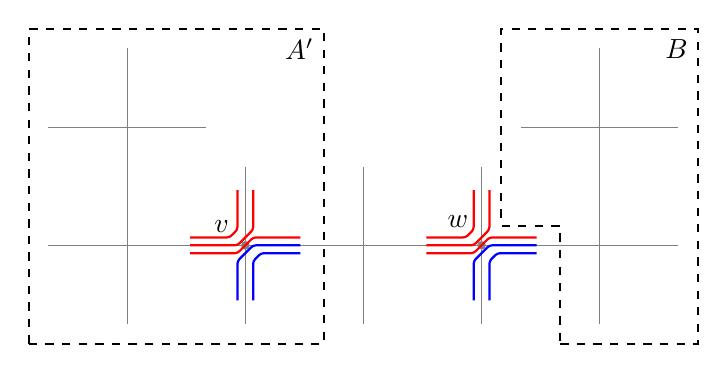
\begin{tikzpicture}[scale=1]

\begin{scope}[gray] % Frame for Wh(X)
  \draw (-4,0) -- (4,0);
  \draw (-4,1.5) -- (-2,1.5);
  \draw (2,1.5) -- (4,1.5);
  \draw (-3,-1) -- (-3,2.5);
  \draw (-1.5,-1) -- (-1.5,1);
  \draw (0,-1) -- (0,1);
  \draw (1.5,-1) -- (1.5,1);
  \draw (3,-1) -- (3,2.5);
\end{scope}

\begin{scope} %vertex labels
  [disc/.style={circle,draw=gray,fill=gray,very thin,inner sep=0pt,minimum
    size=1mm}]
  \node at (-1.80,0.24) {\(v\)};
  \node at (1.20,0.30) {\(w\)};
  \node at (-1.5,0) [disc] {};
  \node at (1.5,0) [disc] {};
\end{scope}

\begin{scope}[thick,rounded corners=1pt] %coloured line patterns
  \foreach \x in {-1.5,1.5} {
    \begin{scope}[red] % Red edges in Wh(*)
      \draw (-0.7+\x,0.1) -- (-0.2+\x,0.1) -- (-0.1+\x,0.2) -- (-0.1+\x,0.7);
      \draw (-0.7+\x,0) -- (-0.1+\x,0) -- (0.1+\x,0.2) -- (0.1+\x,0.7);
      \draw (-0.7+\x,-0.1) -- (-0.1+\x,-0.1) -- (0.1+\x,0.1) -- (0.7+\x,0.1);
    \end{scope}

    \begin{scope}[blue] % Blue edges in Wh(*)
      \draw (0.7+\x,-0.1) -- (0.2+\x,-0.1) -- (0.1+\x,-0.2) -- (0.1+\x,-0.7);
      \draw (0.7+\x,0) -- (0.1+\x,0) -- (-0.1+\x,-0.2) -- (-0.1+\x,-0.7);
    \end{scope}
  }
\end{scope}

\begin{scope}[thick,dashed]
  \draw (-4.25,-1.25) rectangle (-0.5,2.75) node[anchor=north east] {\(A'\)};
  \draw (2.5,-1.25) -- (4.25,-1.25) -- (4.25,2.75) -- (1.75,2.75) --
    (1.75,0.25) -- (2.5,0.25) -- cycle;
  \draw (4.25,2.75) node[anchor=north east] {\(B\)};
\end{scope}

\end{tikzpicture}
\caption{
  Vertices $v$ and $w$ are chosen so that $\sigma$ induces the same partition on \Wh{v} as on \Wh{w}.
  Then $\tau$ is an element of $\cH^0(\calU_{A \union g^{-1} B})$ chosen to induce the same partition on \Wh{A'} as $\sigma$ does.}
  \label{fig:cutting}
\end{figure}

We now cancel off the part of $[\sigma]$ supported on $A$.
Let $Y = A' \union g^{-1} B$.
As described above, $\sigma$ induces a partition on the edges of $\Wh{u}$ for each vertex $u$ in $A'$ and $B$, and hence by translation on $\Wh{u}$ for each vertex $u$ in $Y$.
The partitions at $v \in A'$ and the vertex of $g^{-1}B$ adjacent to $v$ are consistent with respect to the attaching map between the two Whitehead graphs, so we obtain a partition of the graph $\Wh{Y}$ into its connected components.
Hence we can define $\tau \in \cH^0(\calU_Y)$ to be a cycle represented by assigning the integer one to one component of $\Wh{Y}$ and zero to the others in a way that agrees at the vertices of $A'$ with the labelling of components represented by $\sigma$.

Then $[\tau]$ is supported on $Y$, which contains at most $|A'| + |B| < |X|$ vertices, and $[\sigma]-[\tau]$ is supported on $(X - A') \union g^{-1}B$, which has fewer vertices than $X$ since $A'$ has more vertices than $B$.
\end{proof}

Therefore $\cH{}^0(\calD)$ admits a finite generating set as an $F$-module and this generating set can be computed from the line pattern: this is equivalent to finding generators for the kernel of the restriction of $d$ to an abelian group of finite rank, which may be done using Smith Normal Form.
Let $[\sigma_1], \dotsc, [\sigma_k]$ be a generating set for $\cH{}^0(\calD)$.
This is equivalent to a surjection $p \colon (\integers F)^k \to \cH^0 ( \calD)$ of $F$-modules.
Let $e_i$ be the $i$\textsuperscript{th} basis vector in the free module, and let it be mapped to $[\sigma_i]$ under $p$.
To complete the computation of a presentation for of $\cH^0(\calD)$ we need an algorithm that computes a generating set for the kernel of $p$.

For each $[\sigma_i]$ let $X_i$ be the support of $[\sigma_i]$.
A general element $x \in (\integers F)^k$ is of the form
\begin{align}\label{eqn:freemodule}
  x = \sum\limits_j\left(\sum\limits_i n_{ij}g_{ij}\right)e_j, \text{where $n_{ij} \in \integers$, $g_{ij} \in F$}.
\end{align}
Define the support of $x$ to be the convex hull
\begin{align}
  \hull \left(\bigunion\limits_{i, j} g_{ij}(X_j)\right).
\end{align}
Note that the support of $px$ is contained in the support of $x$.

We can now state and prove a theorem that shows that the kernel of $p$ is generated by elements of bounded size, in the same way that Proposition~\ref{proposition:generators_0} shows that $\cH{}^0(\calD)$ is generated by elements of bounded size.

\begin{proposition}\label{proposition:relators_0}
  $\ker p$ is generated as an abelian group by elements whose supports have at most $N$ vertices, where $N$ is a computable function of $\calL$ and $n$.
\end{proposition}

\begin{proof}
Our approach here is similar to that in the proof of Proposition~\ref{proposition:generators_0}: we show that---for sufficiently large (computable) $N$---an element of $\ker p$ supported on a set with more than $N$ vertices can be written as the sum of two elements of $\ker p$ supported on strictly smaller sets.

Let $D$ be the maximum of the diameters of the $X_i$.
Choose $L$ such that any subtree of $T$ of diameter at most $2D$ contains at most $L$ vertices.

From the proof of Proposition~\ref{proposition:generators_0} it is clear that in picking a preimage $x$ under $p$ of an element $[\sigma] \in \cH{}^0( \calD)$ it might well be necessary for the support of $x$ to be strictly larger than the support of $[\sigma]$.
We will need to be able to bound the size of the support of $x$ for $[\sigma]$ supported on a set with diameter at most $2D$.
We deal with this first.

With some care, the proof of Proposition~\ref{proposition:generators_0} gives an explicit bound.
At each step, the cochain is split into two pieces, each supported on a set with strictly fewer vertices.
Hence, since $[\sigma]$ is supported on a set with at most $L$ vertices, it can certainly be written as a $\integers$-linear combination of at most $2^L$ elements of our generating set.
So if each generator has at most $M$ vertices, any $[\sigma]$ supported on a set with diameter at most $2D$ has a preimage supported on a set with at most $2^L M$ vertices.
By construction, this set can be taken to be connected.

Let $N$ be large enough that any subtree $X$ of $T$ with at least $N$ vertices contains a vertex $v$ such that the connected components of $X - v$ can be partitioned into two sets with unions $A$ and $B$, so that each of $A$ and $B$ contains at least $2^LM+L$ vertices.
For example, this holds if $X$ is guaranteed to contain an embedded arc of length at least $2(2^LM+L) +1$.
Then suppose that some element $x \in \ker p$ is supported on a subtree $X \subset T$ with at least $N$ vertices.
Let $v$ be a vertex as in the definition of $N$.
Then we aim to divide $x$ as the sum of two smaller relators by cutting at $v$.

The element $x$ is of the form of Equation~\ref{eqn:freemodule} and is such that $g_{ij}X_j \subset X$ for each $i$ and $j$.
Let $A$ and $B$ be the two subsets of $X - v$ as described above, and let $C$ be the ball in $X$ of radius $D$ centred at $v$.
Let $y \in \integers F^k$ be the sum of those summands of $x$ in Equation~\ref{eqn:freemodule} whose supports are contained in $A$.
Then the support of $y$ is a subset of $A$ and the support of $x-y$ is a subset of $B \union C$.

Roughly, $y$ and $x-y$ will be the two desired smaller relators whose sum is $x$.
However $py \neq 0$, so we shall need to add a small correction term.

Since $py = -p(x-y)$, $py$ is supported on $A \intersection (B \union C) = A \intersection C$.
This is a subtree of a tree of diameter $2D$, so by assumption $py$ has a preimage $w$ under $p$ that is supported on a set with at most $2^LM$ vertices.
Then $p(y-w) = 0$ and $x = (y-w) + (x-y+w)$ so it remains to show that $y-w$ and $x-y+w$ have strictly smaller supports than $x$.
But the support of $x$ has $|A| + |B| + 1$ vertices, while $y-w$ and $x-y+w$ are supported on sets with at most $|A| + 2^LM$ and $| B | + |C| + 2^LM$ vertices respectively.
The subtrees $|A|$ and $|B|$ have at least $2^LM + |C|$ vertices, so this completes the proof.
\end{proof}

\begin{proposition} \label{proposition:computable_dimension_zero}
  There is an algorithm that computes a finite presentation for $\cH{}^0(\calD)$.
\end{proposition}

\begin{proof}
Note that $F$ acts on $\integers F^k$ by translation in the sense that if the support of $x \in \integers F^k$ is $X$ then the support of $g\cdot x$ is $g(X)$.
Hence if $N$ is as in the statement of Proposition~\ref{proposition:relators_0} then that proposition shows that $\ker p$ is generated as an $F$-module by those of its elements that are supported on a ball of radius $N$ ball centred at $1$.

In other words, $\ker p$ is generated by its intersection with the set of those $\integers$-linear combinations of translates of the $\{ e_i\}$ by $F$ whose supports are contained in this ball of radius $N$.
To find all such linear combinations is simply to solve a finite dimensional $\integers$-linear equation, which can be done algorithmically, for example using Smith Normal Form.
\end{proof}

\section{Computing \texorpdfstring{$\cH{}^1(\calD)$}{H1(D,Z)}} \label{section:dimension_1_cohomology}

The first cohomology $\cH{}^1(\calU_X)$ is the quotient of $\cC{}^1(\calU_X)$ by $d\cC{}^0(\calU_X)$, since $\cC{}^2(\calU_X)$ is trivial.
Since taking direct limits of families of $\integers$-modules is an exact functor, $\cH{}^1(\calD)$ is also a quotient: the sequence
\begin{center}\begin{tikzpicture}[>=angle 90]
\matrix (a) [matrix of nodes, row sep=3em, column sep = 2em, text height =
  1.5ex, text depth=0.25ex]
{
  $0$ &
  $d\directlimit_X\cC{}^0(\calU_X,
    \integers)$ &
  $\directlimit_X \cC^1( \calU_X, \integers
   )$ &
  $\cH{}^1(\calD)$ &
  $0$ \\
};
\path[->](a-1-1) edge (a-1-2)
  (a-1-2) edge (a-1-3)
  (a-1-3) edge (a-1-4)
  (a-1-4) edge (a-1-5);
\end{tikzpicture}\end{center}
is exact.
Here we use the fact that for $X \subset X'$ there is a \emph{canonical} refinement map $\calU_{X'} \to \calU_X$.
As in the previous section, each of these abelian groups can be endowed with the structure of an $F$-module so that the homomorphisms in the short exact sequence are homomorphisms of $F$-modules.

Now finding a presentation for $\cH{}^1(\calD)$ is equivalent to finding a presentation for $\directlimit_X \cC^1( \calU_X)$ and a generating set for $d\varinjlim_X\cC{}^0(\calU_X)$.
We present an algorithm that does the former in Proposition~\ref{proposition:one_cocycles_computable} and an algorithm that does the latter in Lemma~\ref{lemma:image}.

As in the previous section, cochains have a convenient representation in terms of the Whitehead graph.
A 1-cochain (with respect to an open cover $\calU$) is a map that associates an integer to each pair $U_1, U_2 \in \calU$ with $U_1 \intersection U_2 \neq \emptyset$.
Equivalently, if $\calU_X$ is the open cover associated to a Whitehead graph $\Wh{X}$, this is the assignment of an integer to each edge in the Whitehead graph, with the restriction that if two edges connect the same pair of vertices then they are assigned the same integer.
Refinement to the open cover associated to a larger Whitehead graph preserves the labelling of the old edges, and assigns the integer zero to each new edge.

\begin{proposition}\label{proposition:one_cocycles_computable}
  The direct limit\/ $\directlimit_X\cC{}^1(\calU_X)$ is isomorphic as an $F$-module to $\integers\calL$ with $F$-action induced by the action of $F$ on the set $\calL$ of lines.
\end{proposition}

\begin{proof}
  We define a map $\theta \from\integers\calL \to \directlimit_X\cC{}^1(\calU_X)$.
  Given a line $l$, choose a subtree $X\subset T$ large enough that no line in $\calL$ except $l$ connects the same two components of $T - X$ that $l$ does.
  Then let $\theta(l)$ be the element of $\cC{}^1(\calU_X)$ represented by labelling the line $l$ in $\Wh{X}$ with the integer one and all other lines with the integer zero.
  Note that the image of $l$ under this map is independent of the chosen subtree of $T$ satisfying the condition, so we obtain a map $\integers\calL\to\cC{}^1(\calU_X)$.

  From the description of all elements of $\directlimit_X\cC{}^1(\calU_X)$ in terms of Whitehead graphs we see that this map is surjective.
  From the description of the refinement maps in terms of Whitehead graphs we see that the map is injective, and it is clearly $F$-equivariant.
\end{proof}

\begin{remark}\label{remark:one_cocycles_presentation}
  We can give an explicit presentation for the $F$-module $\integers\calL$.
  Let $\calL$ be generated by the words $\{w_i\}_{i=1}^n$ and let $\widehat{w_i}$ be the unique element of $F$ such that $w_i$ is a power of $\widehat{w_i}$ and $\widehat{w_i}$ is not a proper power.
  Then $\integers\calL \isom \bigdirectsum_i \integers (F/ \langle \widehat{w_i}\rangle)$.
\end{remark}

Proposition~\ref{proposition:one_cocycles_computable} and Remark~\ref{remark:one_cocycles_presentation} describe the $F$-module $\directlimit\cC{}^1 (\calU_X)$ of one dimensional cocycles.
The cohomology $\cH{}^1( \calD)$ is the quotient of this module by the image under the boundary map of $\directlimit\cC{}^0(\calU_X)$, so it remains to show that this image has a computable generating set.

\begin{lemma}\label{lemma:image}
  The $F$-module $d\directlimit_X\cC{}^0(\calU_X)$ is generated by $d\cC{}^0(\calU_{\{1\}})$. This abelian group is generated by the images under $d$ of the cochains given by assigning the value one to one of the $2\mod{S}$ sets in $\calU_{\{1\}}$ and zero to the others.
\end{lemma}

\begin{proof}
The cochain module $\cC{}^0(\calU_X)$ is generated as an abelian group by those elements that are contained in $\cC{}^0(\calU_{\{1\}})$ for some vertex $v$ of $T$, and is therefore generated as an $F$-module by those of its elements that are contained in $\cC{}^0(\calU_{\{1\}})$.
It follows that $d\directlimit_X\cC{}^0(\calU_X)$ is generated as an $F$-module by $d\cC{}^0(\calU_{\{1\}})$.
The claim concerning the generators of $d\cC{}^0(\calU_{\{1\}})$ is clear.
\end{proof}

Putting the results of this section along with Proposition~\ref{proposition:computable_dimension_zero} we obtain the following Theorem.

\begin{theorem}\label{theorem:decomposition_cohomology_computable}
  There is an algorithm that, when given a free group $F$ and a finite collection of elements of that group, computes presentations for the $F$-modules $\cH{}^k(\calD)$, where $\calD$ is the associated decomposition space.
\end{theorem}

\section{The cohomology of hyperbolic graphs of free groups}\label{section:graphs_of_free_groups}

In this section we apply Theorem~\ref{theorem:decomposition_cohomology_computable} to prove Theorem~\ref{theorem:intro_cech_cohomology_graph_of_groups}: we prove the computability of the \vCech{} cohomology of Gromov boundaries of those hyperbolic groups that are fundamental groups of graphs of free groups with cyclic edge groups.
By Bestvina and Feighn's combination theorem~\cite{bestvinafeighn92}, these are precisely those fundamental groups of finite graphs of free groups with cyclic edge groups that do not contain a Baumslag--Solitar subgroup.
By a theorem of Bestvina and Mess~\cite{bestvinamess91} this proves the computability of the group cohomology of such a group with coefficients in the group ring.
We do this geometrically: we build the boundary of such a group out of the decomposition spaces of the free vertex groups with line patterns generated by the incident edge groups.

In dimension zero an algebraic approach describes the cohomology in greater generality.
In dimensions at least two one can easily prove topologically that the cohomology must vanish.
The most complicated part of the proof of Theorem~\ref{theorem:intro_cech_cohomology_graph_of_groups} is the computability of the cohomology in dimension one.
It has very recently been shown by Manning and Wang~\cite{manningwang18} that the cohomology of the Bowditch boundary of a relatively hyperbolic group is equal to the group cohomology of the group relative to its peripheral subgroups.
In light of this, one could alternatively try to relate the cohomology of a hyperbolic fundamental group of a graph of free groups to the cohomology of the decomposition spaces of its vertex groups algebraically using a group cohomological Mayer-Vietoris argument.

\subsection{Boundaries of fundamental groups of graphs of groups}

Let $G$ be a hyperbolic group and let $T$ be a minimal $G$-tree such that all edge stabilisers are quasi-convex.
Then by~\cite[Proposition 1.2]{bowditch98}, for each vertex $v$ of $T$, $G_v$ is quasi-convex in $G$ and is therefore finitely generated and hyperbolic.
The inclusion $G_v \mapsinto G$ extends to a map $\boundary G_v \to \boundary G$ with image $\Lambda G_v$ and this map is a homeomorphism onto its image.
Then by~\cite[Proposition 1.3]{bowditch98} $\boundary G$ has the following description.
\begin{align}\label{equation:boundary_union}
  \boundary G = \bigunion_{v \in V(T)} \Lambda G_v \disjointunion \boundary T
\end{align}
Furthermore, whenever an edge $e$ separates vertices $v_1$ and $v_2$ in $T$, $\Lambda G_{v_1} \intersection \Lambda G_{v_2} \subset \Lambda G_e$ with equality when $v_1 = \initial(e)$ and $v_2 = \terminal(e)$.
We now aim to give a topological description of $\boundary G$ in terms of the subspaces $\{\Lambda G_v \suchthat v \in V(T)\}$.

Let $X$ be a finite subtree of $T$.
Now define the subset $\boundary_X$ of $\boundary G$ as follows.
\begin{align}
  \boundary_X = \left.\bigunion_{v \in V(X)} \Lambda G_v \middle/\sim \right..
\end{align}
Here $\sim$ is the equivalence relation generated by letting $x\sim y$ whenever $\{x,y\} \subset \Lambda G_e$ for some edge $e \in E(T)$ with $\initial(e) \in X$ and $\terminal(e) \notin X$.

We specialise to two classes of edge stabilisers.

\subsubsection{Infinite cyclic edge stabilisers}

First consider the case in which all edge stabilisers are  infinite cyclic and $G$ is one-ended.
Then for any edge $e \in T$, $\Lambda G_e$ is a cut pair.
Therefore there is a natural map $\boundary G \to \boundary_X$ obtained by, for each edge $e$ of $T$ with $\initial(e) \in X$ and $\terminal(e) \notin X$, collapsing the union of $\Lambda G_e$ with a component of $\boundary G - \Lambda G_e$ to a point: for each such edge $e$, let $T_e$ be the component of $T - \interior e$ containing $\terminal(e)$; then we collapse to a point following set.
\begin{align}
  \bigunion_{v \in V(T_e)} \Lambda G_v \disjointunion \boundary T_e
\end{align}
Call this map $q_X$.

Note that when $X_1 \subset X_2$ are finite subtrees of $T$, $q_{X_1}$ factors through $q_{X_2}$: denote by $p_{X_1,X_2}$ the map $\boundary_{X_2} \to \boundary_{X_1}$ obtained by collapsing $q_{X_2}(\Lambda G_v)$ to a point for each vertex $v \in V(X_2) - V(X_1)$.
Then $q_{X_1} = p_{X_1, X_2} \composed q_{X_2}$.

From this discussion we see that $\boundary G$ admits a natural map to the inverse limit $\inverselimit_X \boundary_X$ of the system $(\{\boundary_X\}_X, \{p_{X_1, X_2}\})$ partially ordered by inclusion of subtrees.
From the decomposition of $\boundary G$ described by Equation~\ref{equation:boundary_union} we see that this map is a bijection.
Each space is compact Hausdorff, so the map is a homeomorphism.

\subsubsection{Trivial edge stabilisers}

Secondly, we perform a similar construction in the case in which all edge stabilisers are trivial.
Here we must assume that $G_v$ is infinite for each vertex $v$.
In this case, for any finite subtree $X$ of $T$, $\boundary_X$ is simply a union
\begin{align}
  \bigunion_{v \in V(X)} \Lambda G_v.
\end{align}
This subset of $\boundary G$ has the topology of the disjoint union of the sets $\{\Lambda G_v \suchthat v \in V(X)\}$.

We now define retracts $q_X \from X \to \boundary_X$.
For each vertex $v \in T$ choose a point $z_v \in \Lambda G_v$.
Now for each edge $e \in E(X)$ such that $\initial(e) \in X$ and $\terminal(e) \notin X$ let $T_e$ be the component of $T - \interior e$ containing $\terminal(e)$ and map the following subset of $\boundary_X$ to the point $z_{\initial(e)} \in \boundary_X$.
\begin{align}
  \bigunion_{v \in V(T_e)} \Lambda G_v \disjointunion \boundary T_e
\end{align}

Then, as in the case of infinite cyclic edge stabilisers, we realise $\boundary G$ as an inverse limit $\inverselimit_X \boundary_X$ of the system $(\{\boundary_X\}, \{p_{X_1, X_2}\})$.

In either case, using the fact that \vCech{} cohomology is a continuous contravariant functor we obtain a description of the \vCech{} cohomology group $\cH{}^k(\boundary G)$.

\begin{proposition}\label{proposition:cech_cohomology_of_graph_of_groups}
  If $G$ is a hyperbolic group and $T$ is a minimal $G$-tree such that either all edge stabilisers are trivial and all vertex stabilisers are infinite, or all edge stabilisers are infinite cyclic, then we have the following isomorphism.
  \begin{align}
    \cH{}^k(\boundary G) \isom \directlimit_X \cH{}^k(\boundary_X)
  \end{align}
\end{proposition}

\subsection{Computing the cohomology}

We now use Proposition~\ref{proposition:cech_cohomology_of_graph_of_groups} to describe the cohomology of $\boundary G$ in terms of the vertex groups.

\subsubsection{Groups with more than one end}

First, we apply Proposition~\ref{proposition:cech_cohomology_of_graph_of_groups} in the case when the edge stabilisers are trivial and the vertex stabilisers are infinite.
Assume also that $G$ is torsion free.
In this case we have observed that $\boundary_X\subset \boundary G$ is a disjoint union $\bigdisjointunion_{v \in V(X)} \Lambda G_v$.
We split into cases: first we treat the cohomology in dimension zero, then in dimensions at least one.
Let $T$ be a Dunwoody decomposition for $G$. Since $G$ is torsion free this coincides with the Grushko decomposition.

In dimension zero, $\cH{}^0(\boundary_X) \isom \bigdirectsum_{v \in V(X)} \cH{}^0(\Lambda G_v)$, but the inclusion $\cH{}^0(\Lambda G_v) \to \cH{}^0(\boundary_X)$ does not coincide with the map $p_{\{v\}, X}^\star$, so we cannot conclude that $\cH{}^0(\boundary G)$ is a direct sum indexed by $V(T)$.
Instead we describe the cohomology in terms of the edges of $T$.
Let $E^{+}(T)$ be a $G$-invariant orientation on $T$: that is, a choice of one element from each pair $\{e, \bar{e}\}$ such that if $e \in E^{+}(T)$ then $g\cdot e \in E^{+}(T)$ for all $g$ in $G$.
We define a map from $\integers E^{+}(T)$ to $\directlimit_X \cH{}^k(\boundary_X)$.
Choose a base point $v \in T$ and let $y = \sum_i n_i e_i \in \integers E^{+}(T)$.
Then for any subtree $X$ of $T$ containing $e_i$ for each $i$, define the image of $y$ in $\cH{}^0(\boundary_X)$ to be given by the following assignment of integers to connected components of $\boundary_X$.
For $w \in X$, assign to $\Lambda G_w$ the sum of the coefficients in $y$ of the edges traversed in the path from $v$ to $w$ in $T$, with edges traversed in the opposite direction counting negatively.
The composition of this map with the map $q_X^\star$ is independent of the choice of $X$, so gives a homomorphism of abelian groups $\integers E^{+}(T) \to \cH{}^0(\boundary G)$.

The map constructed in the previous paragraph depends on choice of base point $v$, and therefore cannot provide an isomorphism of $G$-modules.
However, the induced map $\integers E^{+}(T) \to \cH{}^0_\rmr(\boundary G)$ to the \emph{reduced} cohomology is an isomorphism of abelian groups and does not depend on the base point.
Injectivity of this map follows from the fact that for any edge $e$ of $T$, $G_e$ is an infinite index subgroup of $G_{\initial(e)}$.
It is clear that this map is $G$-equivariant with respect to the $G$-action on $\integers E^{+}(T)$.
All edge stabilisers are trivial, so $\integers E^{+}(T) \isom (\integers G)^{\mod{E(G\backslash T)}}$.
Finally, note that the map $\cH{}^0(\boundary G) \to \cH{}^0_\rmr(\boundary G)$ splits, so $\cH{}^0(\boundary G) \isom \cH{}^0_\rmr(\boundary G) \directsum \integers$, where $G$ acts trivially on $\integers$.

This gives the following proposition. 

\begin{proposition}\label{proposition:0th_cohomology_from_dunwoody_decomposition}
  Let $G$ be a one-ended hyperbolic group.
  Let $T$ be a tree on which $G$ acts minimally such that all edge stabilisers are trivial and all vertex stabilisers are infinite.
  Then $\cH{}^0(\boundary G) \isom (\integers G)^{\mod{E(G\backslash T)}} \directsum \integers$.
\end{proposition}

\begin{remark}
  Algebraic analogues of this statement are true more generally.
  See, for example, \cite[Section 13.5]{geoghegan08}.
\end{remark}

In dimension $k \geq 1$ the situation is simpler: if $e$ is an edge of $X$ and $A$ and $B$ are the two components of $X - \interior e$ then $\cH{}^k(\boundary_X) \isom \cH{}^k(\boundary_A) \directsum \cH{}^k(\boundary_B)$ where the inclusions $\cH{}^k(\boundary_A) \to \cH{}^k(\boundary_X)$ and $\cH{}^k(\boundary_B) \to \cH{}^k(\boundary_X)$ coincide with the maps $p_{A,X}^\star$ and $p_{B,X}^\star$.
It follows that $\cH{}^k(\boundary G) \isom \bigdirectsum_{v \in V(T)}\cH{}^k(\Lambda G_v)$ as abelian groups for $k \geq 1$.

The $G$-action is clear: if $g \in G_v$ then the action of $g$ fixes $\cH{}^k(\Lambda G_v) \subset \cH{}^k(\boundary G)$ and the action on this subspace coincides with the action induced by the action of $g^{-1}$ on $\Lambda G_v$.
If $g \notin G_v$ then the the action of $g^{-1}$ on $\boundary G$ maps $g(\Lambda G_v) = \Lambda G_{gv}$ homeomorphically onto $\Lambda G_v$, so the action of $g$ on $\cH{}^k(\boundary G)$ maps $\cH{}^k(\Lambda G_v)$ isomorphically onto $\cH{}^k(\Lambda G_{gv})$.
Therefore $\cH{}^k(\boundary G)$ is isomorphic as a $G$-module for $k \geq 1$ to the following direct sum.
\begin{align}\label{equation:finite_edge_group_direct_sum}
  \bigdirectsum_{[v] \in V(G\backslash X)} \left(\integers G \tensorproduct_{\integers G_v} \cH{}^k(\boundary G_v)\right)
\end{align}

This argument reduces the problem to the case in which $G$ is one-ended: let $\calY$ be a Dunwoody decomposition of $G$, which may be computed using~\cite{dahmanigroves08a}, and suppose that every vertex group in $\calY$ is infinite.
Then the cohomology of $G$ in dimension zero is given by Proposition~\ref{proposition:0th_cohomology_from_dunwoody_decomposition}, while the cohomology in higher dimensions is given in terms of the one-ended vertex groups by Equation~\ref{equation:finite_edge_group_direct_sum}.

\subsubsection{Groups with one end}

Now suppose that $G$ is one-ended, that stabilisers of vertices in $T$ are free and that the stabilisers of edges in $T$ are cyclic.
We now describe $\cH{}^k(\boundary_X)$ in terms of the limit sets of stabilisers of vertices in $X$.
Let $e$ be an edge of $X$ and let $A$ and $B$ be the two components of $X - \interior e$.
Let $\widehat{\boundary_A}$ be $q_X(\bigunion_{v \in V(A)} \Lambda G_v) \subset \boundary_X$, so that $\boundary_A$ is obtained from $\widehat{\boundary_A}$ by identifying the two points in $\Lambda G_e$.
Similarly define $\widehat{\boundary_B}$, so $\boundary_X = \widehat{\boundary_A} \union \widehat{\boundary_B}$.

Note that the Mayer-Vietoris exact sequence may be applied to the union $\boundary_X = \widehat{\boundary_A} \union \widehat{\boundary_B}$.
This is non-trivial: $\widehat{\boundary_A}$ and $\widehat{\boundary_B}$ are not open in $\boundary_X$ and $\widehat{\boundary_A} \intersection \widehat{\boundary_B}$ is not a strong neighbourhood deformation retract in either $\widehat{\boundary_A}$ or $\widehat{\boundary_B}$.
The exactness of the Mayer-Vietoris sequence for this union is a special feature of \v{C}ech cohomology: \v{C}ech cohomology satisfies a very strong excision property with the consequence that any compact triad is a proper triad with respect to \v{C}ech cohomology, and therefore there is a Mayer-Vietoris exact sequence for any compact triad $(Y, Y_1, Y_2)$ with $Y = Y_1 \union Y_2$.
For more details see~\cite[Chapter 10]{eilenbergsteenrod52}.

For dimension $k > 1$ the Mayer-Vietoris theorem tells us that we have the following isomorphism.
\begin{align}
  \cH{}^k(\boundary_X) \isom \cH{}^k(\widehat{\boundary_A}, \Lambda G_e) \directsum \cH{}^k(\widehat{\boundary_B}, \Lambda G_e) \isom \cH{}^k(\boundary_A) \directsum \cH{}^k(\boundary_B).
\end{align}
Applying this repeatedly we reduce to a direct sum of groups $\cH{}^k(\boundary_{\{v\}})$, where $v$ is a vertex of $X$.
But $\boundary_{\{v\}}$ is simply a decomposition space, so the cohomology in dimensions $k > 1$ vanishes.
Therefore $\cH{}^k(\boundary_X) = 0$ for all finite subgraphs $X$, so $\cH{}^k(\boundary G) = 0$.

In dimension one, the map $\boundary_X \to \boundary_A$ maps $\widehat{\boundary_B}$ to a point, so its restriction to $\widehat{\boundary_B}$ is trivial in first cohomology.
Therefore the following diagram commutes.
\begin{center}
\begin{tikzpicture}
  \matrix (m) [matrix of math nodes, row sep=3em,column sep=3em,minimum width=2em]
  {
    \cH{}^1(\boundary_A) & \cH{}^1(\widehat{\boundary_A}) \\
    \cH{}^1(\boundary_X) & \cH{}^1(\widehat{\boundary_A}) \directsum \cH{}^1(\widehat{\boundary_B}) \\};
  \path[-stealth]
    (m-1-1) edge (m-1-2) edge node [left] {$p_{A,X}^\star$} (m-2-1)
    (m-1-2) edge (m-2-2)
    (m-2-1) edge (m-2-2);
\end{tikzpicture}
\end{center}
Here the map $\cH{}^1(\widehat{\boundary_A}) \to \cH{}^1(\widehat{\boundary_A}) \directsum \cH{}^1(\widehat{\boundary_B})$ is the obvious inclusion map.

Note that $\cH{}^1(\boundary_A) \isom \cH{}^1(\widehat{\boundary_A}, \Lambda G_e)$, so the Mayer-Vietoris exact sequence applied to $\boundary_X = \widehat{\boundary_A} \union \widehat{\boundary_B}$ and the long exact sequences associated to the pairs $(\widehat{\boundary_A}, \Lambda G_e)$ and $(\widehat{\boundary_A}, \Lambda G_e)$ give the following commutative diagram, in which rows are exact sequences.
\begin{center}
\begin{tikzpicture}
  \matrix (m) [matrix of math nodes,row sep=3em,column sep=3em,minimum width=2em]
  {
   \cH{}^0_\rmr(\widehat{\boundary_A})                                                &                           & \cH{}^1(\boundary_A) & \cH{}^1(\widehat{\boundary_A})                                 &   \\
   \cH{}^0_\rmr(\widehat{\boundary_A}) \directsum \cH{}^0_\rmr(\widehat{\boundary_B}) & \cH{}^0_\rmr(\Lambda G_e) & \cH{}^1(\boundary_X)              & \cH{}^1(\widehat{\boundary_A}) \directsum \cH{}^1(\widehat{\boundary_B}) & 0 \\
   \cH{}^0_\rmr(\widehat{\boundary_B})                                                &                           & \cH{}^1(\boundary_B) & \cH{}^1(\widehat{\boundary_B})                                 &   \\};
  \path[-stealth]
    (m-1-1) edge (m-2-1) edge (m-2-2)
    (m-3-1) edge (m-2-1) edge (m-2-2)
    (m-2-1) edge (m-2-2)
    (m-2-2) edge (m-1-3.west) edge (m-2-3.west) edge (m-3-3.west)
    (m-1-3) edge (m-1-4) edge node [right] {$p_{A,X}^\star$} (m-2-3)
    (m-3-3) edge (m-3-4) edge node [right] {$p_{B,X}^\star$} (m-2-3)
    (m-2-3) edge (m-2-4)
    (m-1-4) edge (m-2-4)
    (m-3-4) edge (m-2-4)
    (m-1-4.east) edge (m-2-5)
    (m-2-4.east) edge (m-2-5)
    (m-3-4.east) edge (m-2-5);
\end{tikzpicture}
\end{center}

Let $M$ be the pushout of the maps $\cH{}^0_\rmr(\Lambda G_e) \to \cH{}^1(\boundary_A)$ and $\cH{}^0_\rmr(\Lambda G_e) \to \cH{}^1(\boundary_B)$.
The kernel of the map $\cH{}^0_\rmr(\Lambda G_e) \to M$ is the image of the map $\cH{}^0_\rmr(\widehat{\boundary_A}) \directsum \cH{}^0_\rmr(\widehat{\boundary_B}) \to \cH{}^0_\rmr(\Lambda G_e)$.
We therefore see that $M$ fits into the following commutative diagram, in which rows are exact sequences.
\begin{center}
\begin{tikzpicture}
  \matrix (m) [matrix of math nodes,row sep=1em,column sep=3.2em,minimum width=2em]
  {
                                                                                         &                           & M                    &                                                                              &   \\
      \cH{}^0_\rmr(\widehat{\boundary_A}) \directsum \cH{}^0_\rmr(\widehat{\boundary_B}) & \cH{}^0_\rmr(\Lambda G_e) &                      & \cH{}^1(\widehat{\boundary_A}) \directsum \cH{}^1(\widehat{\boundary_B})     & 0 \\
                                                                                         &                           & \cH{}^1(\boundary_X) &                                                                              &   \\};
  \path[-stealth]
  (m-2-1) edge (m-2-2)
  (m-2-2) edge (m-1-3) edge (m-3-3)
  (m-1-3) edge (m-2-4)
  (m-3-3) edge (m-2-4)
  (m-1-3) edge (m-3-3)
  (m-2-4) edge (m-2-5);
\end{tikzpicture}
\end{center}

By the five lemma it follows that $\cH{}^1(\boundary_X) \isom M$ and the isomorphism from $M$ to $\cH{}^1(\boundary_X)$ is induced by the maps $p_{A,X}^\star$ and $p_{B,X}^\star$.

Since the limit set of an edge stabiliser consists of precisely two points, $\cH{}^0_\rmr(\Lambda G_e) \isom \integers$ for any edge $e \in E(T)$.
For each edge $e \in E(T)$ choose a generator for $\cH{}^0_\rmr(\Lambda G_e)$ equivariantly with respect to the $G$-action on $T$: if $x_e$ is the image in $\boundary G$ of the chosen generator of $\cH{}^0_\rmr(\Lambda G_e)$ then we require that $g\cdot x_e = x_{ge}$ for any $g \in G$.
(Here we use the fact that $G$ is torsion free, so $G_e$ acts trivially on $\Lambda G_e$. If infinite dihedral edge stabilisers were allowed then we would have to be more careful.)

Therefore we see that, as an abelian group, $\cH{}^1(\boundary G)$ is the quotient of $\bigdirectsum_{v \in V(T)}\cH{}^1(\boundary_{\{v\}})$ obtained by identifying the image of the chosen generator of $\cH{}^0_\rmr(\Lambda G_e)$ in $\cH{}^1(\boundary_{\{\initial(e)\}})$ with its image in $\cH{}^1(\boundary_{\{\terminal(e)\}})$ for each edge $e \in E(T)$.
Denote by $x_{\initial e}$ the image of the generator in $\cH{}^1(\boundary_{\{\initial(e)\}})$ and by $x_{\terminal e}$ the image of the generator in $\cH{}^1(\boundary_{\{\terminal(e)\}})$

Then we have the following isomorphism of abelian groups.

\begin{align}
  \cH{}^1(\boundary G) \isom \left.\bigdirectsum_{v \in V(T)} \cH{}^1(\boundary_{\{v\}}) \middle/ \langle x_{\initial(e)} - x_{\terminal(e)} \suchthat e \in E(T)\rangle\right.
\end{align}

We now describe the $G$-module structure of $\cH{}^1(\boundary G)$ in terms of the graph of groups $\calY$ associated to $T$.
Let $Y$ be the underlying graph of $\calY$.
Vertex group in $\calY$ are only identified with stabilisers of vertices in $T$ up to conjugacy in $G$.
To remedy this, let $S$ be a maximal subtree of $Y$ and choose a lift $\widetilde{S}$ of $S$ in $T$.
For each vertex and edge of $S$ choose the group labelling that vertex or edge in $\calY$ to be the stabiliser of the lift of that vertex or edge to $\widetilde{S}$.
Denote this lift of a vertex $v$ by $\widetilde{v}$ and the lift of an edge $e$ by $\widetilde{e}$.
For each edge $e$ in $E(Y) - E(S)$ choose a lift $\widetilde{e}$ of $e$ to $T$ such that $\initial(\widetilde{e}) \in \widetilde{S}$ and label $e$ with the stabiliser $\widetilde{e}$.
Also choose an element $g_e \in G$ such that $\terminal(g_e(\widetilde{e})) \in \widetilde{S}$.
Note then that $x_{\terminal(\widetilde{e})} = g_e^{-1}\cdot x_{\terminal(g_e(\widetilde{e}))}$.

We obtain the following isomorphism of $G$-modules.
\begin{align}
  \left.\cH{}^1(\boundary G) \isom \left(\bigdirectsum_{v \in V(Y)} \integers G \tensorproduct_{\integers G_{\widetilde{v}}} \cH{}^1(\boundary_{\{\widetilde{v}\}})\right) \middle/ R\right.
\end{align}
where $R$ is the $G$-submodule generated by the following finite set.
\begin{align}
  \{1 \tensorproduct (x_{\initial(\widetilde{e})} - x_{\terminal(\widetilde{e})}) \suchthat e \in E(S)\} \union \{1 \tensorproduct x_{\initial(\widetilde{e})} - g_e^{-1} \tensorproduct x_{\terminal(g_e\cdot \widetilde{e})}\suchthat e \in E(Y) - E(S)\}
\end{align}

In the case of interest to us, in which all vertex stabilisers in $T$ are free, $\boundary_{\{v\}}$ is precisely the decomposition space associated to the pair $(G_v, \inc v)$, and therefore $\cH{}^1(\boundary_{\{v\}})$ is computable by Theorem~\ref{theorem:decomposition_cohomology_computable}.
Furthermore, $x_{\initial e}$ is simply the generator corresponding to the line spanned by $G_e \leq G_{\initial e}$, which can readily be identified in $\cH{}^1(\boundary_{\{v\}})$.

Finally, note that given a presentation for a one-ended hyperbolic group that is the fundamental group of a graph of free groups with cyclic edge groups, a decomposition of $G$ with free vertex groups and cyclic edge groups can be computed from that presentation.
First compute Bowditch's canonical decomposition for the group using Theorem~\ref{theorem:computing_JSJ_decompositions}.
If this decomposition is trivial consisting of a single vertex in $T_2$ then the boundary of the group is a circle and the \vCech{} cohomology of the boundary is $\integers$ in dimensions zero and one, with trivial $G$-action.
Otherwise, the stabiliser of every vertex in $T_2$ is free.
Bowditch's canonical decomposition can be refined at vertices in $T_2$ to dominate the decomposition with free vertex groups, so every vertex in $T_1 \union T_3$ is elliptic with respect to this decomposition and therefore every vertex group is free.
It follows that every vertex in Bowditch's canonical decomposition has free stabiliser.

Putting the results of this section together, we obtain the following theorem.

\begin{theorem}
  There is an algorithm that takes as input a presentation for a hyperbolic fundamental group $G$ of a graph of groups with free vertex groups and cyclic edge groups and returns presentations for the \vCech{} cohomology $G$-modules of\/ $\boundary G$.
\end{theorem}

\begin{corollary}
  The group cohomology of a hyperbolic fundamental group of a graph of groups with free vertex groups and cyclic edge groups with coefficients in the group ring $\integers G$ can be computed from a presentation of that group.
\end{corollary}

